\section{Generalization of chaotic dynamics}
We begin by defining a general symbol space.
\begin{definition}
	Denote by $\Sigma^{N}$ the symbol space defined as the space of doubly infinite sequences of $N$ symbols (for $N \in \mathbb{N}$), i.e.
\begin{align}
	\boxed{
		\Sigma^{N} = \left\{ s=\ldots s_{-2} s_{-1} \bm{.} s_0s_1s_2 \ldots:\ s_i \in \{0, 1, \ldots, N-1\} \right\}.
	}
\end{align}
\end{definition}

We may constrain this symbol space by constraining which sequences are admissible. This can be done by using a transition matrix $A \in \mathbb{R}^{N \times N}$ with entries $A_{ij}\in \{0,1\}$. Then the constrained symbol space is given by
\begin{align}
	\Sigma_{A}^{N} = \left\{ s \in \Sigma^{N}:\ A_{s_i s_{i+1}} \neq 0,\forall i \right\}.
\end{align}
In the constrained space, consecutive symbols $s_i$ and $s_{i+1}$ must correspond to a 1 in the transition matrix $A$. In other words if the symbol $s_i=k$ then the symbol $s_{i+1}$ must be equal to $j$ such that $A_{kj}=1$.

\begin{ex}[Constrained symbol space]
	To demonstrate how a transition matrix can constrain the symbol space, lets start by examining $\Sigma_{A}^{2}$ for
	\begin{align}
		A =
		\begin{pmatrix}
			1 & 0 \\
			0 & 1
		\end{pmatrix}
		.
	\end{align}
	Be examining the entries of the transition matrix $A$ we find which strings are admissible
	\begin{align*}
		A_{11}=1 \implies& \ldots 00\ldots \quad \textrm{admissible} \\
		A_{12}=0 \implies& \ldots 01\ldots \quad \textrm{inadmissible} \\
		A_{21}=0 \implies& \ldots 10\ldots \quad \textrm{inadmissible} \\
		A_{22}=1 \implies& \ldots 11\ldots \quad \textrm{admissible}. 
	\end{align*}	
	Therefore the set $\Sigma_{A}^{2}$ is comprised only of two elements $\{\overline{0}\bm{.} \overline{0}, \overline{1}\bm{.} \overline{1}\}$. As this space is very simple and only contains fixed points of $\sigma$, no chaos can occur.
\end{ex}

\begin{definition}
	The map
	\begin{align}
		\sigma:\Sigma_{A}^{N}\to \Sigma_{A}^{N};\quad \ldots s_{-1}\bm{.} s_0 \ldots \mapsto \ldots s_{-1} s_0 \bm{.} s_1 s_2 \ldots,
	\end{align}
	is called a \emph{Bernoulli subshift of finite type} (i.e. $N< \infty $) with transition matrix $A$.
\end{definition}
Before more examination of chaos on such constrained spaces, we need to recall a definition from linear algebra.
\begin{definition}
	A matrix $A$ is called \emph{irreducible} if there exists a $k \in \mathbb{N}$ such that $\left(A^{k}\right)_{ij}\neq 0$ for every $i,j\in \{1,\ldots,N\}$.
\end{definition}

\begin{exercise}
Let $A$ denote the transition matrix for a sub-shift $\sigma\colon\Sigma_{A}^{N}\mapsto\Sigma_{A}^{N}$ of finite type on $N$ symbols. 
\begin{enumerate}
\item Show that the number of fixed points of $\sigma$ is equal to $\textrm{tr(}A)$. 
\item Show that the total number of \emph{admissible} $k-$periodic points (i..e, $k-$periodic points whose minimal period may be less than $k$) is equal to $\textrm{tr(} A^{k})$. 
\end{enumerate}
\end{exercise}


\begin{theorem}[]
	Assume that $A$ is irreducible, then 
	\begin{enumerate}
		\item $\Sigma_{A}^{N}$ is a Cantor set; and
		\item $\sigma:\Sigma_{A}^{N}\to \Sigma_{A}^{N}$ is a chaotic map.
	\end{enumerate}
\end{theorem}

Note that in the previous example with $A=I_{2}$, the transition is not irreducible, which is why chaos is not guaranteed.

The role of irreducibility is critical for the theorem to work. Say for instance that the required $k$ such that each entry of $A^{k}$ is nonzero is $k=3$. Then we know that $\left(A^{3}\right)_{ij} = \sum_{l,m=1}^{N} a_{il}a_{lm}a_{mj} \neq 0$ for any pair $i,j$. Therefore there exist $l,m$ such that $a_{il}$, $a_{lm}$, and $a_{mj}$ which are not equal to 0. Hence there exists an admissible ultimate transition from state $i$ to state $j$ for all pairs $i,j$, if the symbol sequence is viewed as an itinerary. Furthermore, different irreducible transition matrices generate different types of chaos. 

\begin{ex}[Chaos in the Newton-Raphson iteration]
	Newton-Raphson iteration is a process to find the roots (zeros) of a nonlinear function $f$. The iteration is as follows
	\begin{enumerate}
		\item Start with the seed point $x_0$;
		\item Define $x_1 = x_0 - \frac{f(x_0)}{f'(x_0)}= N(x_0)$;
		\item Repeat (ii) as $x_{n+1} = x_n - \frac{f(x_n)}{f'(x_n)}$, until convergence, i. e. until $x_{n+1}=x_n$.
	\end{enumerate}
	In practice this approach is often truncated when $x_{n+1}\approx x_{n}$. The roots of $f$ coincide with the fixed points of the 1-dimensional dynamical system $x_{n+1}= N(x_n)$. If such a fixed point $\overline{x}$ is stable \underline{and} $x_0 $ is in its domain of attraction, then $\lim_{i\to \infty }N^{i}(x_0)= \overline{x}$. The iteration process is sketched in Fig. \ref{fig:NR_iteration}.
\begin{figure}[h!]
	\centering
	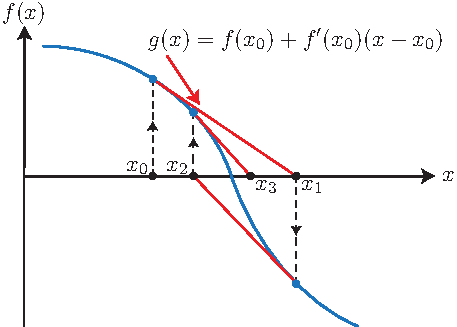
\includegraphics[width=0.6\textwidth]{figures/ch7/1NR_iteration.pdf}
	\caption{An illustration of the iteration of the Newton-Raphson process on the function $f$ (blue). The red designates the function $g$, when given the point $x_0$ the next iterate $x_1$ fufills the property $g(x_1)=0$.}
	\label{fig:NR_iteration}
\end{figure}

Note that if $N(\overline{x}) = \overline{x}$ then we have
\begin{align}
	N'(\overline{x}) = 1 - \frac{f'(\overline{x})^{2} - f(\overline{x})f''(x_0)}{f'(\overline{x})^{2}}=0.
\end{align}
The latter equality is due to $f(\overline{x}) = 0$. Stability of $\overline{x_0}$ clearly follows, because $|N'(\overline{x_0})|<1$. Additionally, since $N'(\overline{x_0})=0$, we call the fixed point \emph{super-stable}.

Specifically, once we are near the optimum $\overline{x}$, we have
\begin{align}
	N(x_n) = \underbrace{N(\overline{x})}_{=\overline{x}} + \underbrace{N'(\overline{x})}_{=0}(x_n - \overline{x}) + \frac{1}{2} N''(\overline{x})(x_n - \overline{x})^{2} + \mathcal{O}\left( | x_n - \overline{x}|^{3}\right).
\end{align}
This implies we have fast quadratic convergence, as
\begin{align}
	\left| N(x_n) - N(\overline{x}) \right| \approx \frac{1}{2} | N''(\overline{x})| |x_{n} - \overline{x}|^{2}.
\end{align}
Despite the fast convergence, erratic iterations may result if the initial point is not close enough to the root \cite{SaariUrenko}. In particular, consider a 4th order polynomial 
\begin{align}
	f(x) = (x-x_0)(x-x_1)(x-x_2)(x-x_3);\quad x_0<x_1<x_2<x_3.
\end{align}
This can be observed to lead to chaotic Newton-Raphson iterations. The proof will be sketched for this chaotic behaviour.

Retain the 4th order polynomial $f$ from above. We then have $N(x_i)=x_i$ for $i=0,1,2,3$ as these are roots of $f$. Note then that we already know what the shapes of $f$ and $f'$ are, and these are illustrated in Fig. \ref{fig:NR_pf1}.
\begin{figure}[h!]
	\centering
	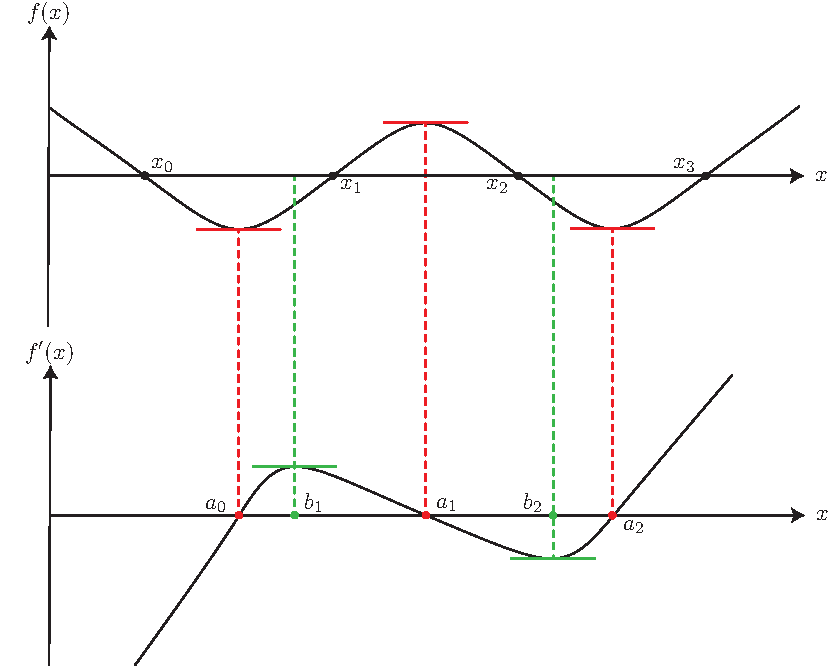
\includegraphics[width=0.9\textwidth]{figures/ch7/2NR_pf1.pdf}
	\caption{The shape of $f$ (above) and $f'$ (below). The points $a_i$ are roots of $f'$ and the points $b_{i}$ are roots of $f''$.}
	\label{fig:NR_pf1}
\end{figure}

The points $a_i$ denote the minima and maxima of $f(x)$ and $b_i$ denote the minima and maxima of $f'(x)$ (See Fig. \ref{fig:NR_pf1}). As $f'(a_i)=0$ we also have that $|N(a_i)|=\infty $, also $f''(b_i)=0$ implies that $N'(b_i)=0$. Thus via our knowledge of the shape of $f$, we have been able to derive information about $N$. If we assume that $b_1\in (a_0, x_1)$ and $b_2\in (x_2, a_2)$, then we get the graph of $N$ as shown in Fig. \ref{fig:NR_graph1}.
\begin{figure}[h!]
	\centering
	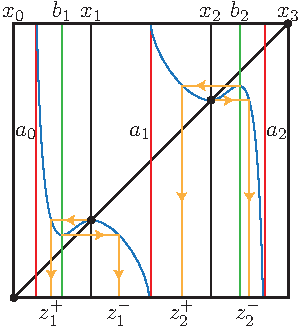
\includegraphics[width=0.5\textwidth]{figures/ch7/3NR_graph1.pdf}
	\caption{The graph of $N$, the points $z_{i}^{\pm}$ are lower bounds on the domain of attraction as they surely converge to the fixed points. The are chosen by starting at a local extrema and working backwards.}
	\label{fig:NR_graph1}
\end{figure}

Next, we seek non-convergent iterations in $[a_0, a_1] \cup [a_1, a_2]$. We begin by finding the preimages of $a_0$ (called $y_{0,i}$) and $a_2 $ (called $y_{2,i}$) this can be done geometrically by starting from the point $a_k$, going down to the diagonal, and then searching horizontally for where the graph of $N$ crosses the level $a_k$; going down from this point to the $x$-axis yields a preimage. This is shown in Fig. \ref{fig:NR_preimages}. Using these points define the following sets
\begin{align}
	I_{1} = [y_{2,1}, z_{1}^{+}];\quad
	I_{2} = [z_{1}^{-}, y_{0,1}];\quad
	I_{3} = [y_{2,2}, z_{2}^{+}];\quad
	I_{4} = [z_{2}^{-}, y_{0,2}].
\end{align}
These sets are illustrated in Fig. \ref{fig:NR_preimages} as well.
\begin{figure}[h!]
	\centering
	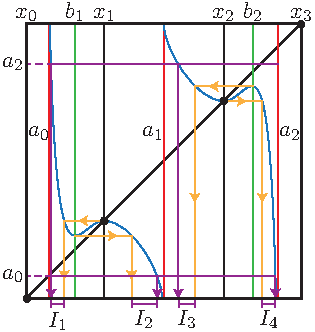
\includegraphics[width=0.5\textwidth]{figures/ch7/4NR_preimages.pdf}
	\caption{The preimages of the values $a_0$ and $a_2$, along with the sets $I_{j}$ for $j=1,2,3,4$.}
	\label{fig:NR_preimages}
\end{figure}

Noting that $b_2 > N(b_2)$ and $b_1 < N(b_1)$ observe that the following hold
\begin{subequations}
\begin{align}
	N(I_1) = [x_1, a_2] \supset I_2 \cup I_3 \cup I_4&; \quad	
	N(I_3) = [N(b_2), a_2] \supset [b_2, a_2] \supset I_4;\\
	N(I_2) = [a_0, N(b_1)] \supset [a_0, b_1] \supset I_1&;\quad
	N(I_4) = [a_0, x_2] \supset I_1 \cup I_2 \cup I_3.
\end{align}
\end{subequations}
\end{ex}
Therefore we have that the possible transitions from $I_{i}$ to $I_{j}$ are described by the transition matrix
\begin{align}
	A = 
	\begin{pmatrix}
		0 & 1 & 1 & 1 \\
		1 & 0 & 0 & 0 \\
		0 & 0 & 0 & 0 \\
		1 & 1 & 1 & 0 \\
	\end{pmatrix}
.	
\end{align}
This transition matrix is in fact irreducible with $k=3$
\begin{align}
	A^2 = 
	\begin{pmatrix}
		2 & 1 & 1 & 1 \\
		0 & 1 & 1 & 1 \\
		1 & 1 & 1 & 0 \\
		1 & 1 & 1 & 2 \\
	\end{pmatrix}
;\quad	
	A^3 = 
	\begin{pmatrix}
		2 & 3 & 3 & 3 \\
		2 & 1 & 1 & 1 \\
		1 & 1 & 1 & 2 \\
		3 & 3 & 3 & 2 \\
	\end{pmatrix}
	.
\end{align}

We are not done yet, as we still need to establish a unique encoding. Note that if $a^{3}_{ij}\neq 0$ then the set $I_{i}\cap f^{-1}(I_j)\neq \emptyset$ is closed for $i=1,2,3,4$. In light of this, with $\tilde{N}=N^3$, define
\begin{subequations}
\begin{align}
	I_{s_0s_1 \ldots s_n} &= I_{s_0} \cap \tilde{N}^{-1}(I_{s_1}) \cap \tilde{N}^{-2}(I_{s_2}) \cap \ldots \cap \tilde{N}^{-n}(I_{s_n}) \\
			      &= I_{s_0} \cap \tilde{N}^{-1}\left(I_{s_1} \cap \tilde{N}^{-1}\left( I_{s_2} \cap \ldots \tilde{N}^{-1}\underbrace{\left(I_{s_{n-1}}\cap \tilde{N}^{-1}(I_{s_n})\right) }_{\neq\emptyset \textrm{, closed} }\right) \right).
\end{align}
\end{subequations}
The condition $I_{s_{n-1}}\cap \tilde{N}^{-1}(I_{s_n})\neq \emptyset$ and is closed is true as each entry $a^{3}_{ij}\neq 0$. Therefore we have a nested sequence of nonempty, closed sets and by Cantor's Theorem their intersection yields a nonempty, closed set. By our previous result we have that $\Lambda= \bigcup_{s\in \Sigma^{N}_{A}}I_{s}$ is a Cantor set. In this case $N=4$ and $A$ is as above. We then have the encoder function $\phi:\Lambda \to \Sigma_{A}^{4}$ and the chaotic function $\sigma:\Sigma_{A}^{4}\to \Sigma_{A}^{4}$. These yield the commuting diagram
\begin{equation}
\begin{tikzcd}
	\Sigma_{A}^{4} \arrow[r, "\sigma"] 
& \Sigma_{A}^{4} \\
\Lambda \arrow[u,"\phi"] \arrow[r, "N"]
& \Lambda \arrow[u, "\phi"] 
\end{tikzcd}.
\end{equation}
Thus we have that $N=\phi^{-1}\circ \sigma \circ \phi$, which implies that $N$ is a chaotic map. Hence, the Newton-Raphson iteration has an invariant Cantor set, on which the iteration is equivalent to a Bernoulli subshift of finite type on 4 symbols.
